
% $Header: /cvsroot/latex-beamer/latex-beamer/solutions/generic-talks/generic-ornate-15min-45min.en.tex,v 1.5 2007/01/28 20:48:23 tantau Exp $

\documentclass[smaller]{beamer}
\mode<presentation>
{
  \usetheme{Singapore}
  \usefonttheme[onlymath]{serif}
  % or ...
 %  \setbeamercovered{transparent}
  % or whatever (possibly just delete it)
}

\usepackage{amssymb}
\usepackage[czech]{babel}
% or whatever
\usepackage[utf8]{inputenc}
% or whatever
%\usepackage{times}
%\usepackage[T1]{fontenc}
% Or whatever. Note that the encoding and the font should match. If T1
% does not look nice, try deleting the line with the fontenc.


\title{PAS09\\ Non-parametric tests\\Two sample tests}

\author{Jan B\v rezina}
\institute % (optional, but mostly needed)
{
  %\inst{2}%
  Technical University of Liberec
}


% If you wish to uncover everything in a step-wise fashion, uncomment
% the following command: 

%\beamerdefaultoverlayspecification{<+->}

% ***************************************** SYMBOLS
\def\div{{\rm div}}
\def\Lapl{\Delta}
\def\grad{\nabla}
\def\supp{{\rm supp}}
\def\dist{{\rm dist}}
%\def\chset{\mathbbm{1}}
\def\chset{1}

\def\Tr{{\rm Tr}}
\def\sgn{{\rm sgn}}
\def\to{\rightarrow}
\def\weakto{\rightharpoonup}
\def\imbed{\hookrightarrow}
\def\cimbed{\subset\subset}
\def\range{{\mathcal R}}
\def\leprox{\lesssim}
\def\argdot{{\hspace{0.18em}\cdot\hspace{0.18em}}}
\def\Distr{{\mathcal D}}
\def\calK{{\mathcal K}}
\def\FromTo{|\rightarrow}
\def\convol{\star}
\def\impl{\Rightarrow}
\DeclareMathOperator*{\esslim}{esslim}
\DeclareMathOperator*{\esssup}{ess\,sup}
\DeclareMathOperator{\ess}{ess}
\DeclareMathOperator{\osc}{osc}
\DeclareMathOperator{\curl}{curl}

%\def\Ess{{\rm ess}}
%\def\Exp{{\rm exp}}
%\def\Implies{\Longrightarrow}
%\def\Equiv{\Longleftrightarrow}
% ****************************************** GENERAL MATH NOTATION
\def\Real{{\rm\bf R}}
\def\Rd{{{\rm\bf R}^{\rm 3}}}
\def\RN{{{\rm\bf R}^N}}
\def\D{{\mathbb D}}
\def\Nnum{{\mathbb N}}
\def\Measures{{\mathcal M}}
\def\d{\,{\rm d}}               % differential
\def\sdodt{\genfrac{}{}{}{1}{\rm d}{{\rm d}t}}
\def\dodt{\genfrac{}{}{}{}{\rm d}{{\rm d}t}}

\def\vc#1{\mathbf{\boldsymbol{#1}}}     % vector
\def\tn#1{{\mathbb{#1}}}    % tensor
\def\abs#1{\lvert#1\rvert}
\def\Abs#1{\bigl\lvert#1\bigr\rvert}
\def\bigabs#1{\bigl\lvert#1\bigr\rvert}
\def\Bigabs#1{\Big\lvert#1\Big\rvert}
\def\ABS#1{\left\lvert#1\right\rvert}
\def\norm#1{\bigl\Vert#1\bigr\Vert} %norm
\def\close#1{\overline{#1}}
\def\inter#1{#1^\circ}
\def\ol#1{\overline{#1}}
\def\ul#1{\underline{#1}}
\def\eqdef{\mathrel{\mathop:}=}     % defining equivalence
\def\where{\,|\,}                    % "where" separator in set's defs
\def\timeD#1{\dot{\overline{{#1}}}}

% ******************************************* USEFULL MACROS
\def\RomanEnum{\renewcommand{\labelenumi}{\rm (\roman{enumi})}}   % enumerate by roman numbers
\def\rf#1{(\ref{#1})}                                             % ref. shortcut
\def\prtl{\partial}                                        % partial deriv.
\def\Names#1{{\scshape #1}}
\def\rem#1{{\parskip=0cm\par!! {\sl\small #1} !!}}

\def\Xint#1{\mathchoice
{\XXint\displaystyle\textstyle{#1}}%
{\XXint\textstyle\scriptstyle{#1}}%
{\XXint\scriptstyle\scriptscriptstyle{#1}}%
{\XXint\scriptscriptstyle\scriptscriptstyle{#1}}%
\!\int}
\def\XXint#1#2#3{{\setbox0=\hbox{$#1{#2#3}{\int}$}
\vcenter{\hbox{$#2#3$}}\kern-.5\wd0}}
\def\ddashint{\Xint=}
\def\dashint{\Xint-}

% ******************************************* DOCUMENT NOTATIONS
% document specific
\def\rh{\varrho}
\def\vl{{\vc{u}}}
\def\th{\vartheta}
\def\vx{\vc{x}}
\def\vX{\vc{X}}
\def\vr{\vc{r}}
\def\veta{\vc{\eta}}
\def\dx{\,\d\vx}
\def\dt{\,\d t}
\def\bulk{\zeta}
\def\cS{\close{S}}
\def\eps{\varepsilon}
\def\phi{\varphi}
\def\Bog{{\mathcal B}}
\def\Riesz{{\mathcal R}}
\def\distr{\mathcal D}
\def\Item{$\bullet$}

\def\MEtst{\mathcal T}
%***************************************************************************
\setbeamercolor{my blue}{fg=blue}
\def\blue#1{{\usebeamercolor[fg]{my blue} #1}}

\setbeamercolor{my green}{fg=green}
\def\green#1{{\usebeamercolor[fg]{my green} #1}}

% color for term definition
\setbeamercolor{my orange}{fg=orange}
\def\df#1{{\usebeamercolor[fg]{my orange} #1}}
\def\xskip{{\vspace{2ex}}}

\def\cz#1{{\small (#1)}}

\def\E{\vc{\mathsf{E}}}

\begin{document}

\begin{frame}
  \titlepage
\end{frame}

\begin{frame}{Sign test}
$\{X_1,\dots,X_n\}$ sample from any continuous distribution with median $\tilde{x}$

\xskip
$H_0: \tilde{x} = x_0$,\\
possible $H_A$ (usual): \\
$\tilde{x} \ne x_0$ or $\tilde{x} < x_0$ or $\tilde{x} > x_0$

\xskip
Test procedure:
\begin{enumerate}
 \item remove median values, $X_i = x_0$ (possibly diminishing $n$)
 \item compute statistics $Y$ --- number of cases: $X_i > x_0$
 \item $Y$ has distribution $Bi(n, 1/2)$ (under $H_0$)
\end{enumerate}

\xskip
Note: Not very sensitive to continuity assumption, then Step 1) is necessary.
\end{frame}

\begin{frame}{Sign test (continued)}
Computing  $p$-value
\begin{enumerate}
 \item For small $n$, we can compute $p$-value from definition (e.g. for two side alternative):
  \[
     p=2 \min\{1-F_Y(Y_{obs}), F_Y(Y_{obs})\}, \qquad F_Y(Y) = \sum_{k=0}^{Y} \binom{n}{k} (1/2)^n
  \]
 \item for bigger $n$ we can use equivalence between Binomial and Fisher distribution:
  \[
     F_{Bi(n,p)}(s) = F_{2(n-s),2(s+1)} \Big(\frac{(s+1)(1-p)}{p(n-s)}\Big)
  \]
 \item for big  $n$ (Moivre theorem: $np(1-p) >9$), approximation by normal distribution:
 \[
    U = \frac{Y - np}{\sqrt{np(1-p)}} = \frac{2Y -n}{\sqrt{n}} \sim N(0,1)
 \]
\end{enumerate}

\end{frame}

%TODO: stabilizující transformace


\begin{frame}[fragile]{Wilcoxon test}
$\{X_1,\dots,X_n\}$ sample from continuous distribution,\\
\blue{symmetric} around median $\tilde{x}$, i.e. $f(\tilde{x} + x) = f(\tilde{x} -x)$

\xskip
$H_0: \tilde{x} = x_0$, and classical three alternatives

\xskip
\begin{enumerate}
 \item remove median values: $X_i = x_0$ and denote $Y_i = X_i - x_0$
 \item sort $\{Y_i\}$ by $\abs{Y_i}$
 \item denote $R_i$ rank \cz{pořadí} of value $Y_i$ in sorted sequence
 \item \[
          S^+ = \sum_{Y_i >0} R_i,\qquad  S^- = \sum_{Y_i <0} R_i,\qquad S^+ + S^- = n(n+1)/2
       \]
 \item final statistics is $Y = S^+$
 
\end{enumerate}

\verb'R> psignrank( Y, n=... )'
\end{frame}


\begin{frame}[fragile]{Wilcoxon test (continued)}
 \begin{itemize}
  \item For small values of $Y$:\\
   $H_0$ is rejected in favor $H_A: \tilde{x} \ne x_0$ if $Y \le w_n(\alpha)$ (tables)
  \item For larger $n$ we can use approximation:
  \[
    U = \frac{S^+ - ES^+}{\sqrt{var S^+}} = \frac{12 S}{n(n+1)(2n+1)} \sim N(0,1)
  \]
with mean value and variance:
  \[
    ES^+ = \frac{1}{4}n(n+1),\quad var S^+ = \frac{1}{24}n(n+1)(2n+1)
  \]
  \[
    S = S^+ - S^- = \sum_{i} R_i \sgn Y_i
  \]
 \end{itemize}
 \verb'R> wilcox.test( x, mu=60, exact=T/F )'
\end{frame}


\begin{frame}[fragile]{Example for median tests}
10 persons had to estimate period of 1 minute. $H_0: \tilde{x} = x_0$, $H_A: \tilde{x} < x_0$
\[
 X_i: 53, 48, 45, 55, 63, 51, 66, 56, 50, 58
\]

\begin{enumerate}
  \item Sign test: $Y = 2$, $n=10$:
  \[
    p_{val}= \binom{10}{0} 0.5^{10} +\binom{10}{1} 0.5^{10}+\binom{10}{2} 0.5^{10}=\frac{1}{1024} ( 1 + 10 + 5*9) = 0.055   
  \]
  \verb'R> pbinom(length(x[x>60]),size=length(x), p=0.5)'
%
  \item Wilcoxon test: 
   \[
      X_i-x_0 = -7, -12, -15, -5, 3, -9, 6, -4, -10, -2 
   \]
   \[
      sorted: -2, 3, -4, -5, 6, -7, -9, -10, -12, -15    
   \]
   \[ 
      S^+= 2 + 5 =7;\quad S^- =10*11/2-S^+ = 48;\quad Y=7;\quad p_{val}=0.01855469
   \]

   
    TODO: Sample to small for two side alternative\dots
%  real mearurements of half an minute estimates:
%   39, 29,20,19,26,28,33,21,28,31
\end{enumerate}

\end{frame}


\begin{frame}{Test Kolmogorov-Smirnov}
Test if the sample is from particular distribution.\\

\xskip
\blue{Assumption:}\\
random sample $\{X_0,\dots,X_n\}$ is from continuous distribution

\xskip
  $H_0$ : data $X_n$ has distribution function $F(x)$ (fully given)\\
  $H_A$ : data do not have distribution function $F(x)$
\end{frame}

\begin{frame}[fragile]{Performing K-S test}
  \begin{enumerate}
   \item Compute empirical distribution function $F_n(x)$.
   \item Compute statistics:
   \[
      D_n = \sup_{x} \abs{F_n(x) - F(x)} = \max_{i} \big( \abs{ \frac{i-1}{n} - F(X_n)}, \abs{\frac{i}{n} - F(X_n)} \big)
   \]
   \item For small $n$ compare with tabled critical values $D_n(\alpha)$ (viz skripta Ostrava, Tabulka 5).\\
         $H_0$ is rejected if $D_n \ge D_n(\alpha)$.
   \item For large $n$, we use asymptotic value:
         \[
            D_n^{\star}(\alpha) = \sqrt{\frac{1}{2n} \ln\frac{2}{\alpha}}
         \]
  \end{enumerate}
   \verb'R> ks.test()'
\end{frame}

\begin{frame}[fragile]{Example}
 We are testing an generator of random values with\\
 uniform distribution $U(0,1)$.
\[
X_i: .93, .35, .66, .94, .14, .23, .08, .24, .21, .59
\]
\begin{verbatim}
> x_generator=c( .93, .35, .66, .94, .14, .23, .08, .24, .21, .59)
> ks.test(x_generator, punif)

        One-sample Kolmogorov-Smirnov test

data:  x_generator 
D = 0.26, p-value = 0.4351
alternative hypothesis: two-sided 
\end{verbatim}
\df{tie}: repeated vaules, should not happen for continuous data, but can resoult from rounding, problematic!!
R gives warning for ties.
\end{frame}


\begin{frame}[fragile]{Testing normality}
 \df{ Lilliefors test} - like K-S test, but parameters of normal distribution 
 are given by point estimates $\overline X_n$ a $S_n$. 
% 
 \xskip
 Distribution of statistic is different.
 \begin{verbatim}
  R> install.package(nortest)
  R> library(nortest)
  R> lillie.test(data)
 \end{verbatim}
%
 \xskip
 \df{Shapiro test} - better power, standard
 \verb'shapiro.test(data)'
\end{frame}


\section{Two sample tests}

\begin{frame}[fragile]{Paired $t$-test}
\blue{Example:} Two methods where used to determine content of Fe in $10$ samples.
Results are $X_i$ (first) and $Y_i$ (second method).
Test hypothesis that both methods give the same result (no systematic error).

\xskip
!! $X_i$ and $Y_i$ are dependent r.v. since they corresponds to the same sample, but
we use $Z_i=X_i-Y_i$ and perform $t$-test on the vector $\{Z_i\}$, assuming $Z_i$ has normal distribution

\begin{verbatim}
> x
 [1] 36.1 40.6 35.0 39.3 31.2 38.6 31.8 36.1 36.9 35.2
> y
 [1] 35.2 49.6 38.3 48.6 27.6 39.9 28.5 37.3 35.8 34.3
> x-y
 [1]  0.9 -9.0 -3.3 -9.3  3.6 -1.3  3.3 -1.2  1.1  0.9
> 
\end{verbatim}
\end{frame}

\begin{frame}{other paired tests}
\begin{itemize}
 \item paired Wilcoxon test
 \item
\end{itemize}

\end{frame}


\begin{frame}{two sample $t$-test (same variance)}
\blue{assumpitions:}\\
$X_1, \dots ,X_m$ selection from $N(\mu_1,\sigma_1^2)$,\\
$Y_1, \dots ,Y_n$ selection from $N(\mu_2,\sigma_2^2)$,\\
\blue{$\sigma_1 = \sigma_2$}, test is not too sensitive to this assumption

\xskip
$H_0: \mu_1 - \mu_2  = \delta$ vs. alternatives $H_A: \mu_1 - \mu_2  \lesseqqgtr \delta$

\xskip
under the hypothesis $H_0$ has $T$ Student distribution with $n+m-2$ degrees of freedom:
\[
 T = \frac{\ol{X} - \ol{Y} - \delta}{s_p\sqrt{1/n +1/m}} \sim t_{n+m-2}
\]
where
\[
   s_p = \sqrt{\frac{(n-1)s_X^2 + (m-1)s_Y^2}{n+m-2}},
\]
$\ol{X}, \ol{Y}$ are averages, and $s_X, s_Y$ sample standard deviations.

\blue{$p$-value:} $F_{t_{n+m-2}}(T)$
\end{frame}

\begin{frame}[fragile]{Two sample $t$-test (different variances)}
\dots for case $\sigma_1 \ne \sigma_2$ (big difference),
same hypothesis $H_0$, $H_A$

\blue{Cochran-Cox test}
    \[
      v_X = \frac{s_X^2}{m},\qquad v_Y = \frac{s_Y^2}{n},\qquad S = \sqrt{v_X + v_Y}
    \]
    \[
      T^\star = \frac{\ol{X} - \ol{Y} -\delta}{S},\qquad t^\star = \frac{v_X t_{m-1}(\alpha) + v_Y t_{n-1}(\alpha)}{v_X +v_Y}
    \]
    $H_0$ is rejected in favor of  $H_A: \mu_1 -\mu_2 \ne\delta$ if $\abs{T^\star} \ge t^\star$, no simple $p$-value

\blue{Aspin-Welch test} (used by R, $p$-value possible)\\
   statistics $T^\star$ has approximatively $t_f$ distribution for 
   \[
      f=\frac{S^4}{\frac{v_X^2}{m-1} + \frac{v_Y^2}{n-1}}
   \]

\blue{Satterthwait test} \dots different choice of DoFs
In is necessary to calculate with non-integral degrees of freedom.
\verb'R> t.test(x,y, mu=  , paired=T/F, var.equal=T/F )'
\end{frame}

\begin{frame}{Example}
The new manuring \cz{hnojení} was tried on $8$ fields (with returns $X_i$),\\ 
an old manuring on $5$ fields (returns $Y_i$).

\[
 m=8,\quad n=5,\quad \ol{X}=5.387,\quad \ol{Y}=4.7,\quad s_X^2=0.2698,\quad s_Y^2=0.24
\]
Student's test, $H_A: \mu_X\ne \mu_Y$: \\
$\abs{T}=2.37$ greater then critical value $t_{11}(0.025) =2.201$, rejecting $H_0$, $p_{val} = 0.037 < 0.5$

\xskip
Student's test,  $H_A: \mu_X > \mu_Y$: \\
$T=2.37$ greater then critical value $t_{11}(0.05) =1.796$, rejecting, $p_{val} = 0.019 < 0.5$
\end{frame}

\begin{frame}{\dots using tests for different variances}
Cochran $H_A:  \mu_X\ne \mu_Y$:
$T^{\star} = 2.4$, $t^{\star} = 2.6$, no reject $H_0$
\xskip
Aspin-Welch $f=9.044$, $t_f(0.025) = 2.26$, reject $H_0$, $p_{val} = 0.040$

\xskip
Satterthwait $h=11.086$, $t_h(0.025) =2.2$, reject $H_0$, $p_{val} = 0.035$

\end{frame}




\begin{frame}[fragile]{F-test for ratio of variances }
$X_1, \dots ,X_m$ selection from $N(\mu_1,\sigma_1^2)$,\\
$Y_1, \dots ,Y_n$ selection from  $N(\mu_2,\sigma_2^2)$,\\
$s_X \ge s_Y$ ( simpler performance of the test)

\[
  T=\frac{s_X^2}{s_Y^2} \sim F_{m-1,n-1},
\]
where $F_{M,N}$ is  Fisher-Snedekor distribution.

We reject $H_0:\sigma_1 = \sigma_2$ in favor  $H_A: \sigma_1\ne\sigma_2$ if 
\[
  T \ge F^{-1}_{n-1,m-1}\Big(\frac{\alpha}{2}\Big)
\]

\verb'R>var.test(x, y, ratio= )'
\end{frame}

\begin{frame}{$F$-distibution}
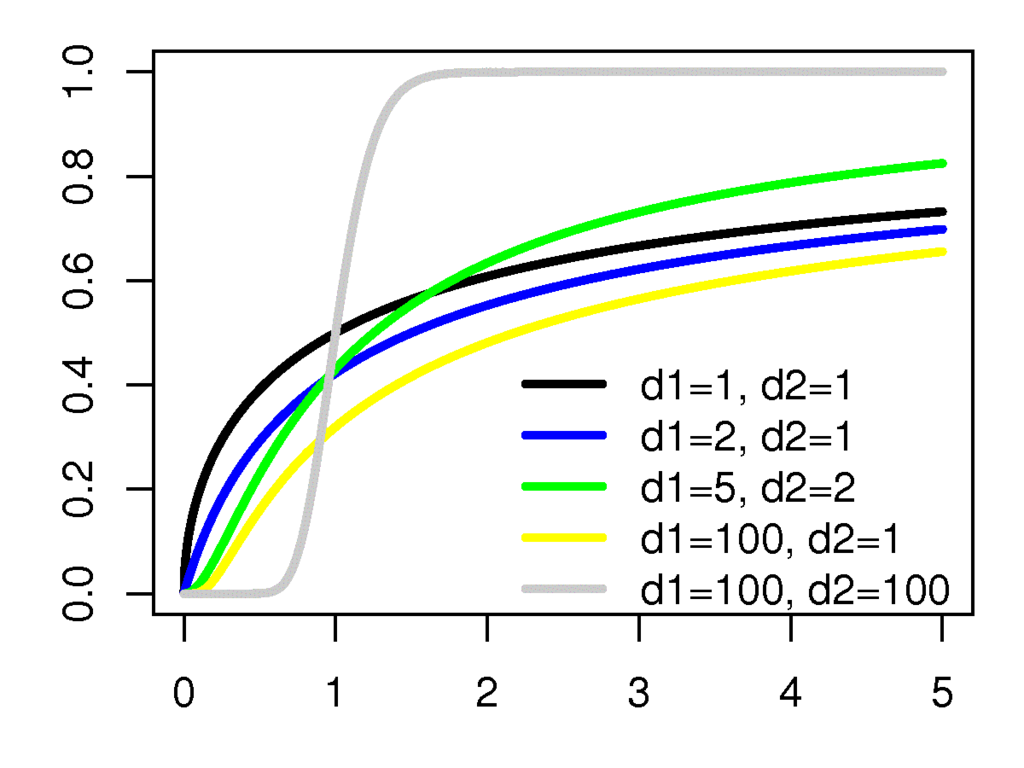
\includegraphics[scale=0.6]{09_F_distributionCDF.png} 
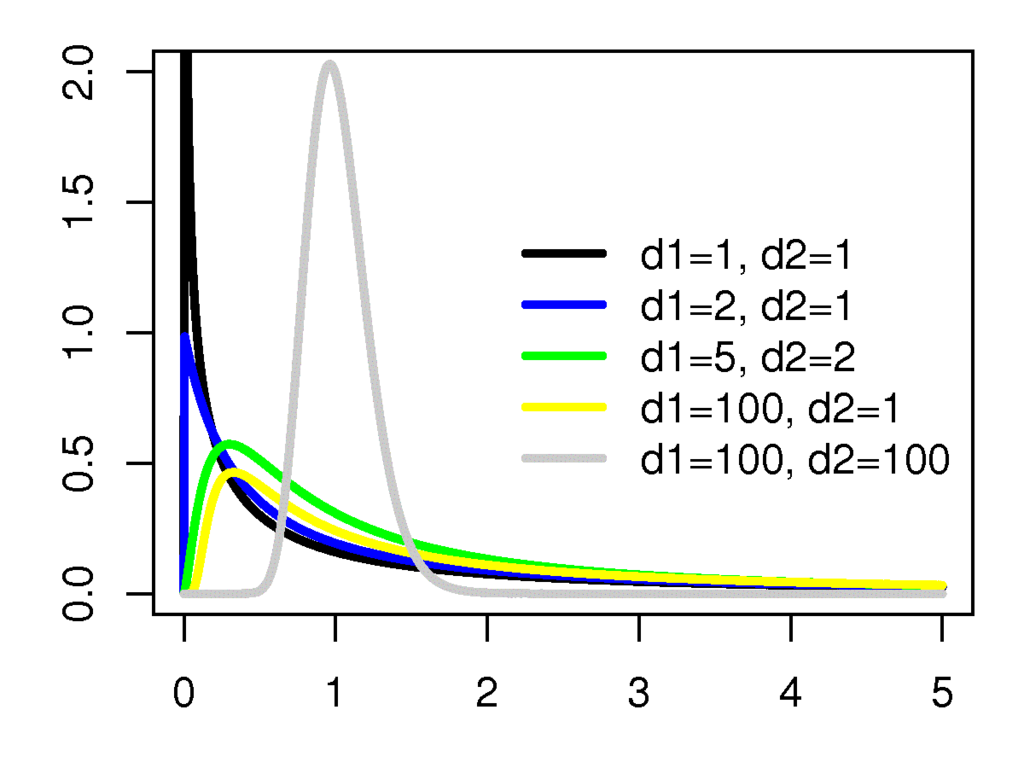
\includegraphics[scale=0.6]{09_F_distributionPDF.png} 
\end{frame}


\begin{frame}[fragile]{$F$-distribution}
Distribution of ratio of two $\chi^2$ random variables.
\[
    \frac{m \chi_n^2}{n \chi_m^2} \sim F_{n,m}
\]
\[
 T=\frac{s^2_X}{s^Y}=\frac{m-1}{n-1} \frac{\frac{s^2_X(n-1)}{\sigma^2}}{\frac{s^2_Y(m-1)}{\sigma^2}} \sim F_{n-1,m-1}
\]


\verb'R> pf( x, df1= , df2= )'

\xskip
\blue{properties:}
\[
 F_{m,n}\Big(1-\frac{\alpha}{2}\Big) = \frac{1}{F_{n,m}\big(\frac{\alpha}{2}\big)}
\]
\end{frame}



\begin{frame}{Example}
\dots setting about manuring \cz{hnojení}: 
\[
 m=8,\quad n=5,\quad s_X^2=0.2698,\quad s_Y^2=0.24
\]
$T = 1.124\quad <\quad F_{7,4}(0.025) = 9.07$,\\
do not reject same variances, $p_{val}=0.52$
 
\end{frame}


\begin{frame}{Relation between binomial and Fisher distribution}
Distribution function of $Bi(n,p)$ can be calculated from $F_{2(n-s),2(s+1)}$:
\[
 F_{Bi}(s) = \sum_{i=0}^s \binom{n}{i} p^i (1-p)^i = F^\star_{2(n-s),2(s+1)}\Big(\frac{(s+1)(1-p)}{p(n-s)}\Big) 
\]
Interval estimate $(L,H)$ for relative frequency $p$, giving sample frequency $Y\sim Bi(n,p)$ (i.e. $Y$ successes from $n$ trials)
\[
 L = \frac{Y}{Y +(n-Y+1)F_{2(n-Y+1),2Y}(\alpha / 2)},
\]
\[
 H = \frac{(Y+1)F_{2(Y+1),2(n-Y)}(\alpha / 2)}{n-Y +(Y+1)F_{2(Y+1),2(n-Y)}(\alpha / 2)}.
\]
\end{frame}


\begin{frame}{Test about equality of proportions, approach A}
$H_0: p_X = p_Y$, 

sample relative frequencies:
\[
 x=\frac{X}{m}\qquad y=\frac{Y}{n}
\]
statistic (approximate each frequency independently):
\[
 U_a = \frac{x-y}{\sqrt{\frac{x(1-x)}{m} + \frac{y(1-y)}{n}}} \quad \sim N(0,1)
\]

$H_0$ is rejected if $U_a \ge u(\alpha / 2)$ 
\end{frame}

\begin{frame}{Test about equality of proportions, approach B}
Approximation of common relative frequency $p_X = p_Y$ ($H_0$ assumption):
\[
 z = \frac{X + Y}{m+n}
\]
statistic:
\[
 U_b = \frac{x-y}{\sqrt{z(1-z)\big(\frac{1}{m} + \frac{1}{n}\big)}} \quad \sim N(0,1)
\]

$H_0$ is rejected if $U_b \ge u(\alpha / 2)$. 
\end{frame}

\begin{frame}[fragile]{Example}
 50 teeth - temperature shocks, 50 - teeth slowly boiled,\\
 21 resp. 11 breaks under mechanical stress. Decide if the 
 shocks has important influence.
 
 \xskip
 Testing one side alternative $p_1 - p_2 >0$:
 $U_a = 2.19,\ p_a=0.014$ and $U_b=2.14,\ p_b=0.016$ 
 \verb'R> prop.test(c(21,11), c(50,50), alternative="gr")'\\
 gives $p=0.027$ !!
\end{frame}


\begin{frame}{Two sample Kolmogorov-Smirnov}
$X_1, \dots ,X_m$ selection from continuous distribution $F$,\\
$Y_1, \dots ,Y_n$ selection from continuous distribution $G$,\\
independent variables

\xskip
$H_0: F=G$ vs. $H_A: F\ne G$\\
Empirical distribution functions $F_m$, $G_n$

\[
 D_{m,n} = \sup_{x}\abs{F_m(x) - G_n(x)}
\]

rejecting $H_0$ if $D_{m,n}$ is greater then $D_{m,n}(\alpha)$, use tables for small $m,n$ viz. Ostravská skripta.
For bigger values, approximation:
\[
 D^\star_{m,n}(\alpha) = \sqrt{\frac{1}{2M} \ln\frac{2}{\alpha}}, \qquad M = \frac{mn}{m+n}
\]
\end{frame}

\end{document}
